\clearpage
\begin{appendices}
	\section{Graph Appendix}
	\label{appendix:graph}
	This is the graph appendix...
	
	\section{Another Appendix}
	
\end{appendices}

	\begin{figure*}[htb]
	\centering
	\caption{Estadisticos de las variables. Elaboración propia}
	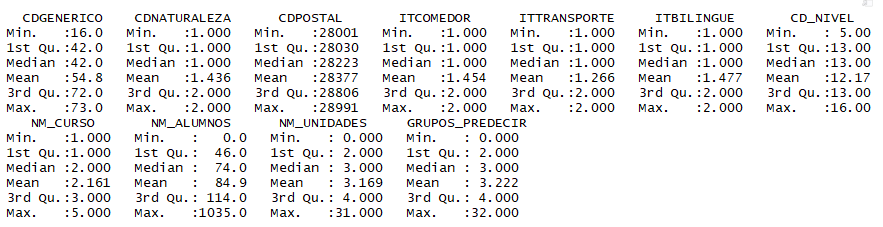
\includegraphics[width=1.2\textwidth]{recursos/ImagenesR/estadisticos}
	\label{fig:estadisticos}
\end{figure*}
\FloatBarrier

	\begin{figure*}[htb]
	\centering
	\caption{Diagrama de cajas. Elaboración propia}
	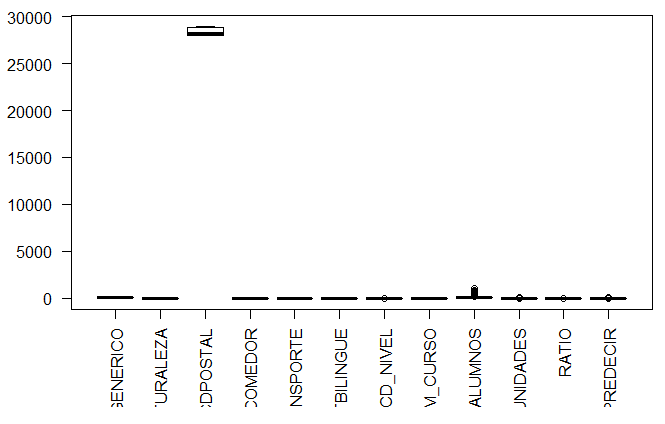
\includegraphics[width=0.8\textwidth]{recursos/ImagenesR/boxplot}
	\label{fig:boxplot}
\end{figure*}
\FloatBarrier


	\begin{figure*}[htb]
	\centering
	\caption{Matriz de correlaciones. Elaboración propia}
	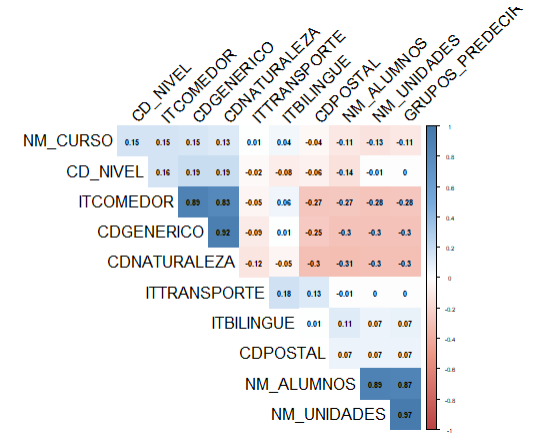
\includegraphics[width=0.8\textwidth]{recursos/ImagenesR/matrizcorrelacion}
	\label{fig:matrizcorrelaciones}
\end{figure*}
\FloatBarrier


	\begin{figure*}[htb]
	\centering
	\caption{Variables mas correladas. Elaboración propia}
	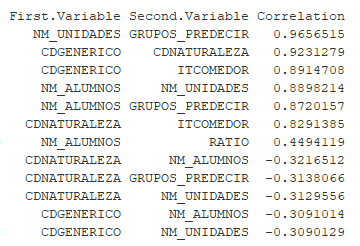
\includegraphics[width=0.6\textwidth]{recursos/ImagenesR/mayorescorrelaciones}
	\label{fig:mayorescorrelaciones}
\end{figure*}
\FloatBarrier

	\begin{figure*}[htb]
	\centering
	\caption{Mayor correlacion con variable a predecir. Elaboración propia}
	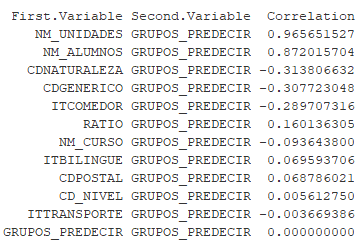
\includegraphics[width=0.6\textwidth]{recursos/ImagenesR/mayorcorrelacion}
	\label{fig:mayorcorrelacionpredecir}
\end{figure*}
\FloatBarrier

	\begin{figure*}[htb]
	\centering
	\caption{Correlación entre variables NM\_ALUMNOS y NM\_GRUPOS. Elaboración propia}
	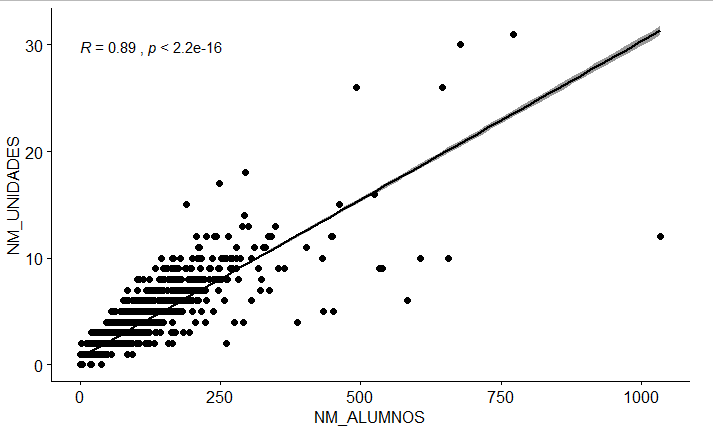
\includegraphics[width=0.6\textwidth]{recursos/ImagenesR/RelacionAlumnGrupos}
	\label{fig:relacionAlumnGrup}
\end{figure*}
\FloatBarrier


	\begin{figure*}[htb]
	\centering
	\caption{Correlación entre variables NM\_ALUMNOS y NM\_GRUPOS. Elaboración propia}
	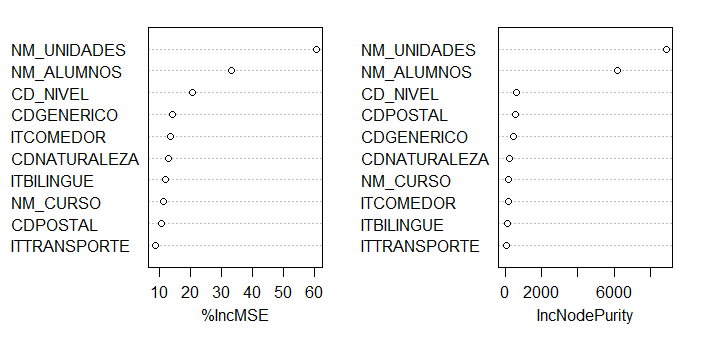
\includegraphics[width=0.6\textwidth]{recursos/ImagenesR/VarImpRF}
	\label{fig:VarImpRF}
\end{figure*}
\FloatBarrier

